\setbeamercolor{background canvas}{bg=tublue}
\begin{frame}
%%%%%%%%%%% TITLE PAGE %%%%%%%%%%%%%%%%%%%%%%%%%%%%%%%%%%%%%%%%%%%%%%%%%%%%%%%%%%%%%%%%%%%%
% 16:10
\Large{
	\vspace{-12mm}
	\hspace{-8mm}
	\begin{minipage}{33.5mm}
		
\includegraphics[width=30mm]{pic/logo/tu_weiss.pdf}
	\end{minipage}\\
% 	\hfill
	\textcolor[rgb]{1.00,1.00,1.00}{
		\begin{minipage}{163mm}%{228mm}
			\setlength{\unitlength}{1mm}
			\begin{picture}(148,8)
				\linethickness{.1mm} \put(-15,7){\line(1,0){165}}
				\put(3.4,4.8){\tiny \textbf{Department of Mathematics~}Institute of Scientific Computing}
				\linethickness{.1mm} \put(-15,4){\line(1,0){165}}
			\end{picture}
		\end{minipage}
		\rule{0pt}{2.3em}
		\begin{center}
			{\huge \textbf{Discrete Exterior Calculus (DEC) for the
      Surface Navier-Stokes Equation}}
		\end{center}
		\rule{0pt}{3.7em}
		\begin{center}
			{\small Ingo Nitschke\\} %\rule{0pt}{1em}%\vspace{1em}
			{\footnotesize \emph{Institute of Scientific Computing}} \\
		\end{center}
		\rule{0pt}{5em}
% 		\tikz[overlay,remember picture]
% 		\node[anchor=center] at ($(current page.center)+(6,-2.5)$) {
% 			{\tiny\emph{Financial support provided by}}
% 		};
% 		\tikz[overlay,remember picture]
% 		\node[anchor=center] at ($(current page.center)+(6,-3.6)$) {
% 			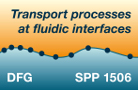
\includegraphics[width=0.2\textwidth]{pic/logo/spp1506.jpg}
% 		};
% 		\tikz[overlay,remember picture]
% 		\node[anchor=center] at ($(current page.center)+(-6,-3.6)$) {
% 			\includegraphics[width=0.2\textwidth]{pic/logo/logo_dfg.jpg}
% 		};
	}
	\thispagestyle{empty}
}

\end{frame}
\setbeamercolor{background canvas}{bg=}
